% Options for packages loaded elsewhere
\PassOptionsToPackage{unicode}{hyperref}
\PassOptionsToPackage{hyphens}{url}
%
\documentclass[
  12pt,
]{article}
\usepackage{amsmath,amssymb}
\usepackage{setspace}
\usepackage{iftex}
\ifPDFTeX
  \usepackage[T1]{fontenc}
  \usepackage[utf8]{inputenc}
  \usepackage{textcomp} % provide euro and other symbols
\else % if luatex or xetex
  \usepackage{unicode-math} % this also loads fontspec
  \defaultfontfeatures{Scale=MatchLowercase}
  \defaultfontfeatures[\rmfamily]{Ligatures=TeX,Scale=1}
\fi
\usepackage{lmodern}
\ifPDFTeX\else
  % xetex/luatex font selection
\fi
% Use upquote if available, for straight quotes in verbatim environments
\IfFileExists{upquote.sty}{\usepackage{upquote}}{}
\IfFileExists{microtype.sty}{% use microtype if available
  \usepackage[]{microtype}
  \UseMicrotypeSet[protrusion]{basicmath} % disable protrusion for tt fonts
}{}
\makeatletter
\@ifundefined{KOMAClassName}{% if non-KOMA class
  \IfFileExists{parskip.sty}{%
    \usepackage{parskip}
  }{% else
    \setlength{\parindent}{0pt}
    \setlength{\parskip}{6pt plus 2pt minus 1pt}}
}{% if KOMA class
  \KOMAoptions{parskip=half}}
\makeatother
\usepackage{xcolor}
\usepackage[margin=1in]{geometry}
\usepackage{graphicx}
\makeatletter
\def\maxwidth{\ifdim\Gin@nat@width>\linewidth\linewidth\else\Gin@nat@width\fi}
\def\maxheight{\ifdim\Gin@nat@height>\textheight\textheight\else\Gin@nat@height\fi}
\makeatother
% Scale images if necessary, so that they will not overflow the page
% margins by default, and it is still possible to overwrite the defaults
% using explicit options in \includegraphics[width, height, ...]{}
\setkeys{Gin}{width=\maxwidth,height=\maxheight,keepaspectratio}
% Set default figure placement to htbp
\makeatletter
\def\fps@figure{htbp}
\makeatother
\setlength{\emergencystretch}{3em} % prevent overfull lines
\providecommand{\tightlist}{%
  \setlength{\itemsep}{0pt}\setlength{\parskip}{0pt}}
\setcounter{secnumdepth}{-\maxdimen} % remove section numbering
\ifLuaTeX
  \usepackage{selnolig}  % disable illegal ligatures
\fi
\usepackage{bookmark}
\IfFileExists{xurl.sty}{\usepackage{xurl}}{} % add URL line breaks if available
\urlstyle{same}
\hypersetup{
  pdftitle={Forecasting Air Quality Index in London},
  pdfauthor={Anusha Bhat, Sarah Chaker, Hritik Jhaveri, John Melel},
  hidelinks,
  pdfcreator={LaTeX via pandoc}}

\title{Forecasting Air Quality Index in London}
\author{Anusha Bhat, Sarah Chaker, Hritik Jhaveri, John Melel}
\date{2025-03-13}

\begin{document}
\maketitle

\setstretch{1.241}
\section{1. Introduction}\label{introduction}

Air pollution is a critical public health concern in urban areas,
particularly in London, where long-term exposure to poor air quality
contributes to respiratory diseases, cardiovascular issues, and reduced
life expectancy. The importance of monitoring and forecasting air
quality in London cannot be overstated, as it directly affects public
health, the economy, and the overall livability of the city. Timely
intervention, such as issuing health advisories, implementing traffic
control measures, and enforcing emissions regulations, can help mitigate
these risks. By forecasting the Air Quality Index (AQI), stakeholders
like the Greater London Authority, UK Environment Agency, Public Health
England, Transport for London, and industrial sectors can make informed
decisions on pollution control, public health strategies, and urban
planning. Additionally, London residents, commuters, and environmental
advocacy groups all stand to benefit from better air quality management.

The data used for this project is sourced from Open-Meteo, an
open-source weather API that provides free access to weather data for
non-commercial use. The dataset contains daily AQI readings for London,
using the USAQI (United States Air Quality Index) scale. This scale is
commonly employed to assess and report air quality levels, reflecting
concentrations of pollutants like particulate matter (PM2.5, PM10),
ozone, and nitrogen dioxide. The data spans from January 2, 2013, to
February 28, 2025, covering a significant period that captures both
long-term trends and seasonal variations in air quality. By leveraging
this dataset, the goal of this project is to develop a time series
forecasting model to predict future AQI levels, enabling stakeholders to
issue early warnings for high pollution days, implement timely pollution
control measures, and guide long-term environmental strategies aimed at
improving air quality, protecting public health, and promoting
sustainable urban development.

\section{2. Data}\label{data}

The dataset used in this study is sourced from Open-Meteo and contains
hourly Air Quality Index (AQI) values for London.

\subsection{2.1 Data Transformation}\label{data-transformation}

The AQI measurements are recorded at an hourly frequency, and few minor
gaps in the data were observed due to occasional missing values. To
address this, linear interpolation was applied to estimate and fill in
the missing hourly values, and following this interpolation step, the
hourly AQI values were aggregated to obtain daily AQI readings, which is
used for the forecasting.

\subsection{2.2 Elementary Data
Analysis}\label{elementary-data-analysis}

The AQI plot for London from 2013 to 2025.
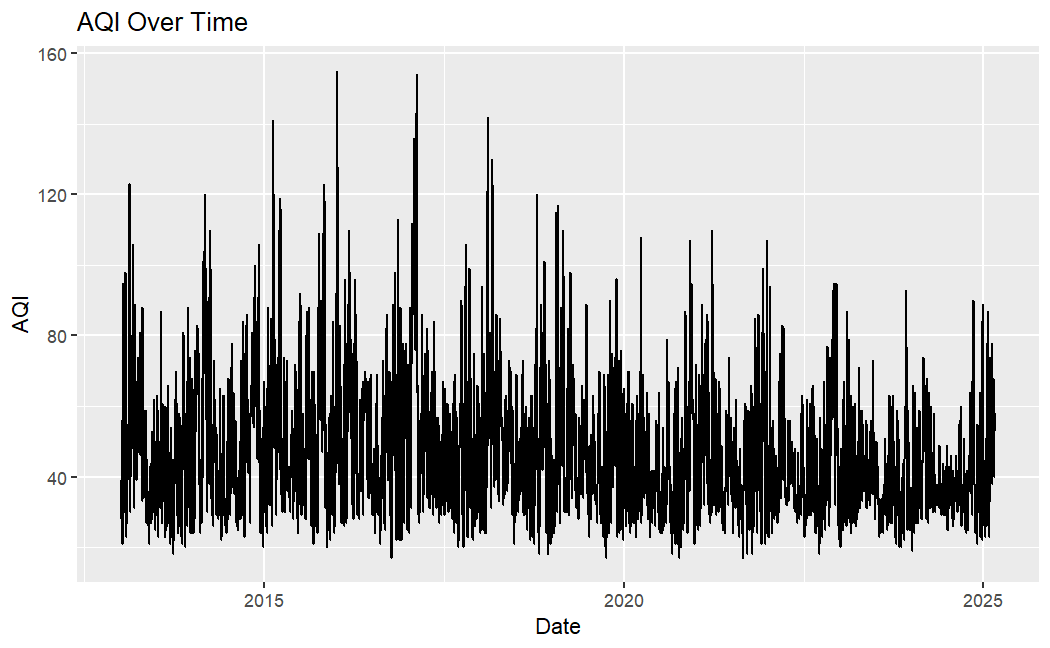
\includegraphics{aqi_plot.png}

ACF Plot: The ACF plot indicates some autocorrelation.


\includegraphics{acf.png}

PACF Plot: The PACF plot indicates some autocorrelation.

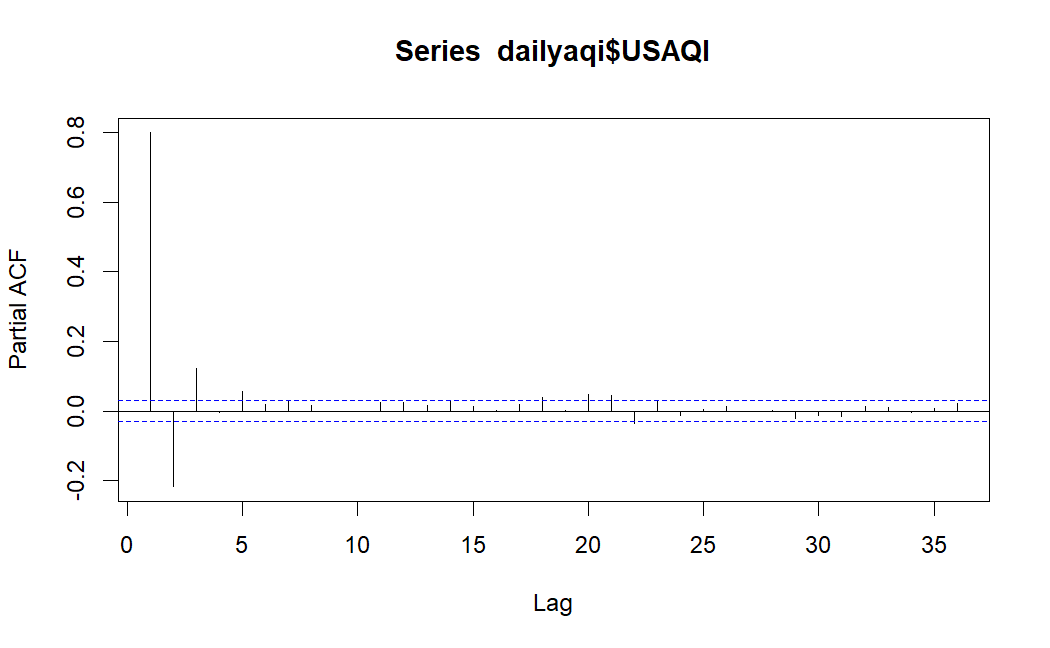
\includegraphics{pacf.png}

STL Decomposition: The STL decomposition shows clear trends and some
yearly seasonality.


\includegraphics{stl.png}

Stationarity tests: We conducted ADF and KPSS test for the data, and
notice ADF test indicating stationarity for the data, but the KPSS test
indicates non-stationarity for the non-differenced data and indicates
stationarity for the differenced data.

Outliers: The AQI values were inspected for outliers. Although some
values deviated significantly from the mean, they were still within a
reasonable AQI range and were retained in the dataset.

Data Citation: Open Meteo
(\url{https://open-meteo.com/en/docs/air-quality-api}) METEO FRANCE,
Institut national de l'environnement industriel et des risques (Ineris),
Aarhus University, Norwegian Meteorological Institute (MET Norway),
Jülich Institut für Energie- und Klimaforschung (IEK), Institute of
Environmental Protection -- National Research Institute (IEP-NRI),
Koninklijk Nederlands Meteorologisch Instituut (KNMI), Nederlandse
Organisatie voor toegepast-natuurwetenschappelijk onderzoek (TNO),
Swedish Meteorological and Hydrological Institute (SMHI), Finnish
Meteorological Institute (FMI), Italian National Agency for New
Technologies, Energy and Sustainable Economic Development (ENEA) and
Barcelona Supercomputing Center (BSC) (2022): CAMS European air quality
forecasts, ENSEMBLE data. Copernicus Atmosphere Monitoring Service
(CAMS) Atmosphere Data Store (ADS).

\section{3. Models}\label{models}

\subsection{3.1 ARIMA, SARIMA, ARFIMA}\label{arima-sarima-arfima}

\subsection{3.2 ETS, Holt Winters}\label{ets-holt-winters}

\subsection{3.3 BSTS}\label{bsts}

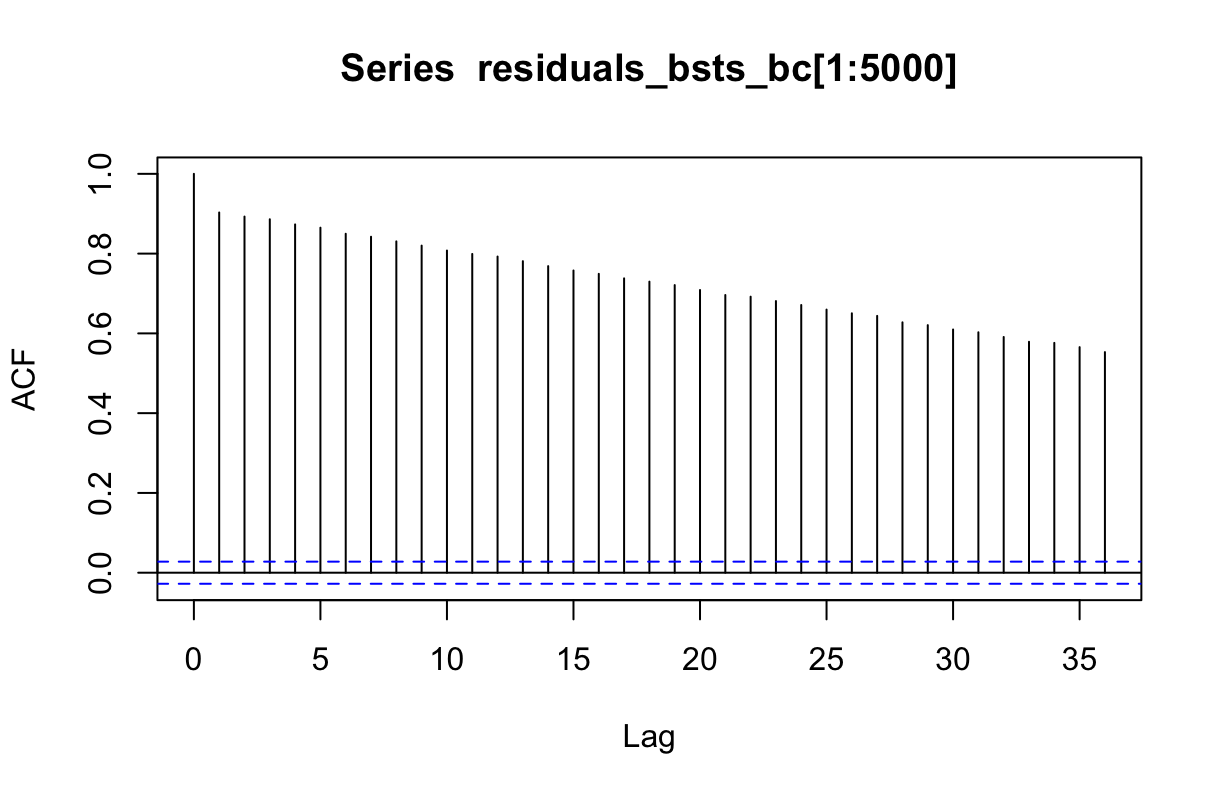
\includegraphics{BSTS_SC/BSTS_bc_acf.png}

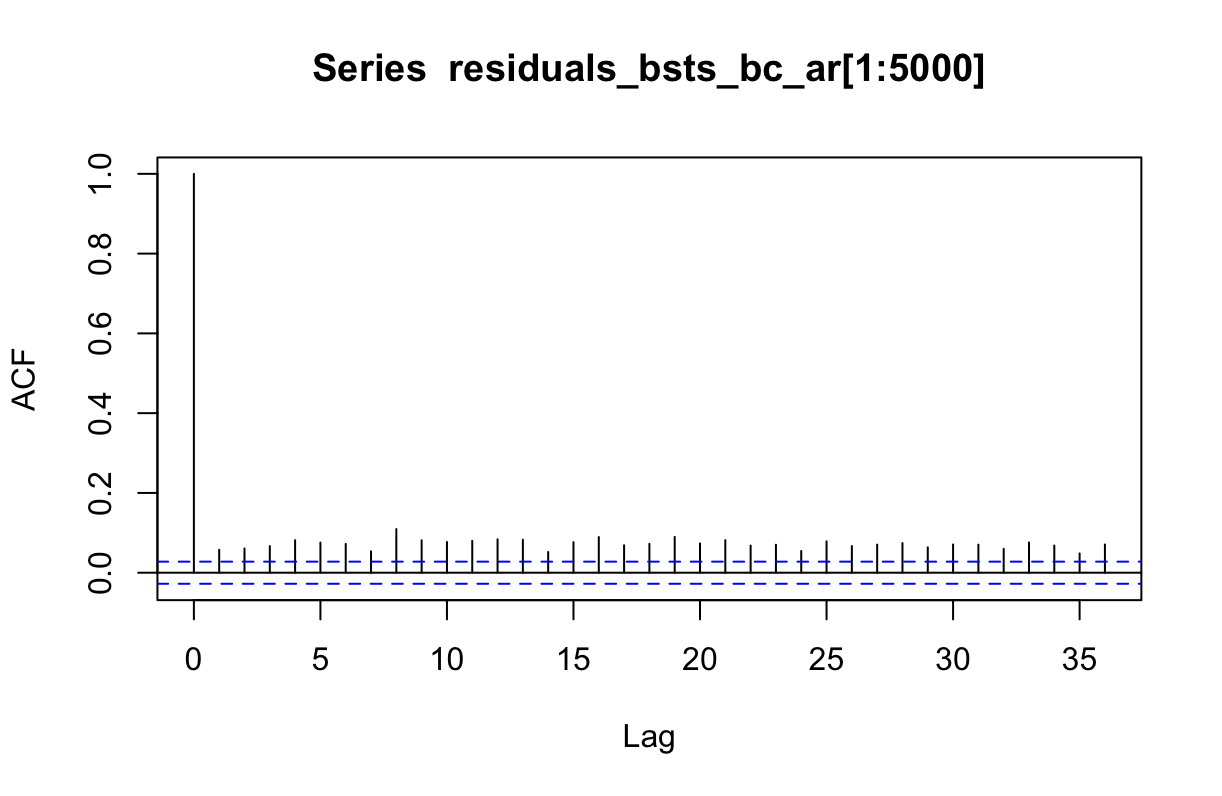
\includegraphics{BSTS_SC/BSTS_bc_ar_acf.png}

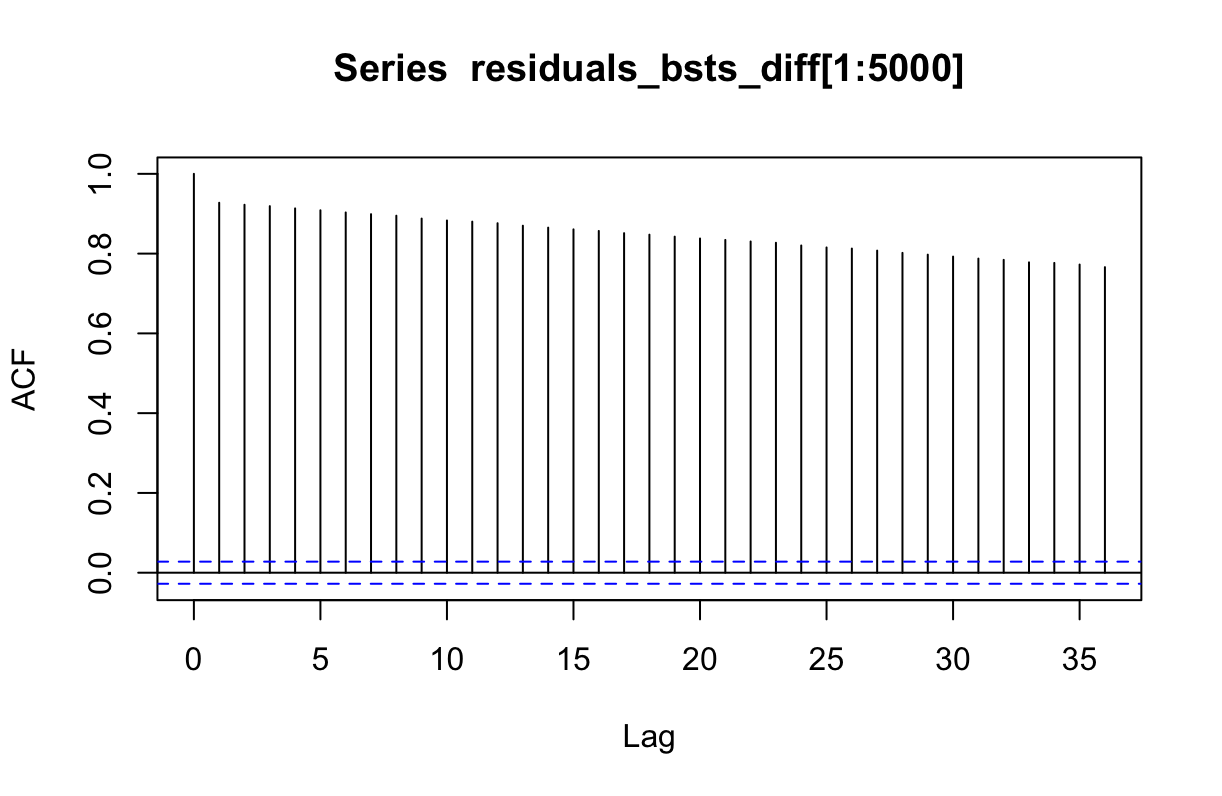
\includegraphics{BSTS_SC/bsts_diff_acf.png}

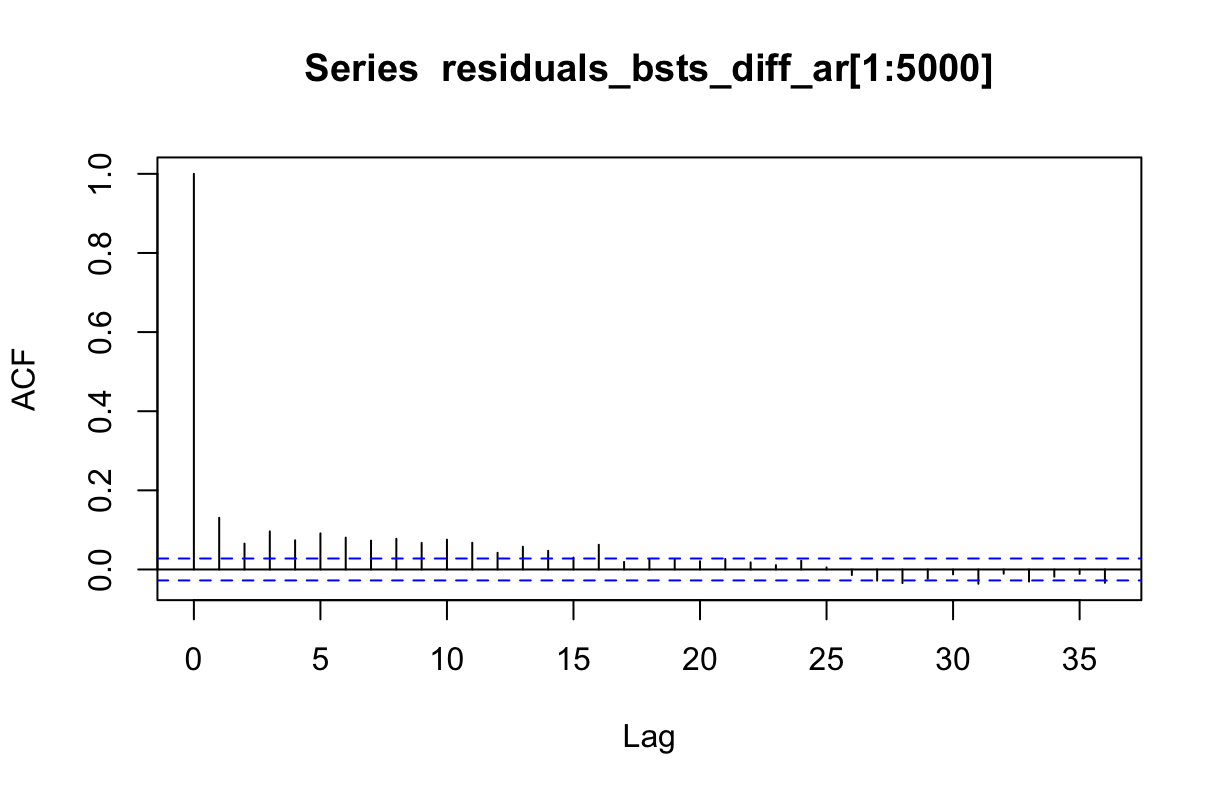
\includegraphics{BSTS_SC/bsts_diff_ar.png}

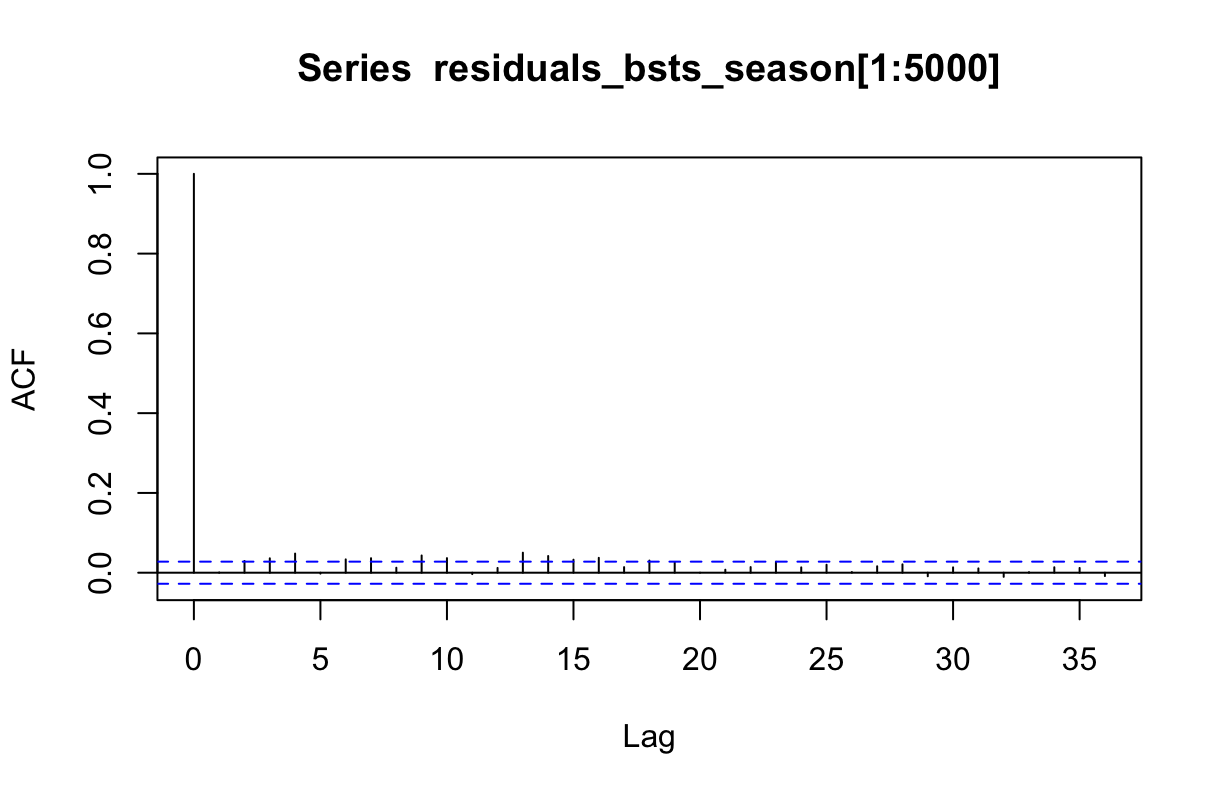
\includegraphics{BSTS_SC/bsts_season_acf.png}

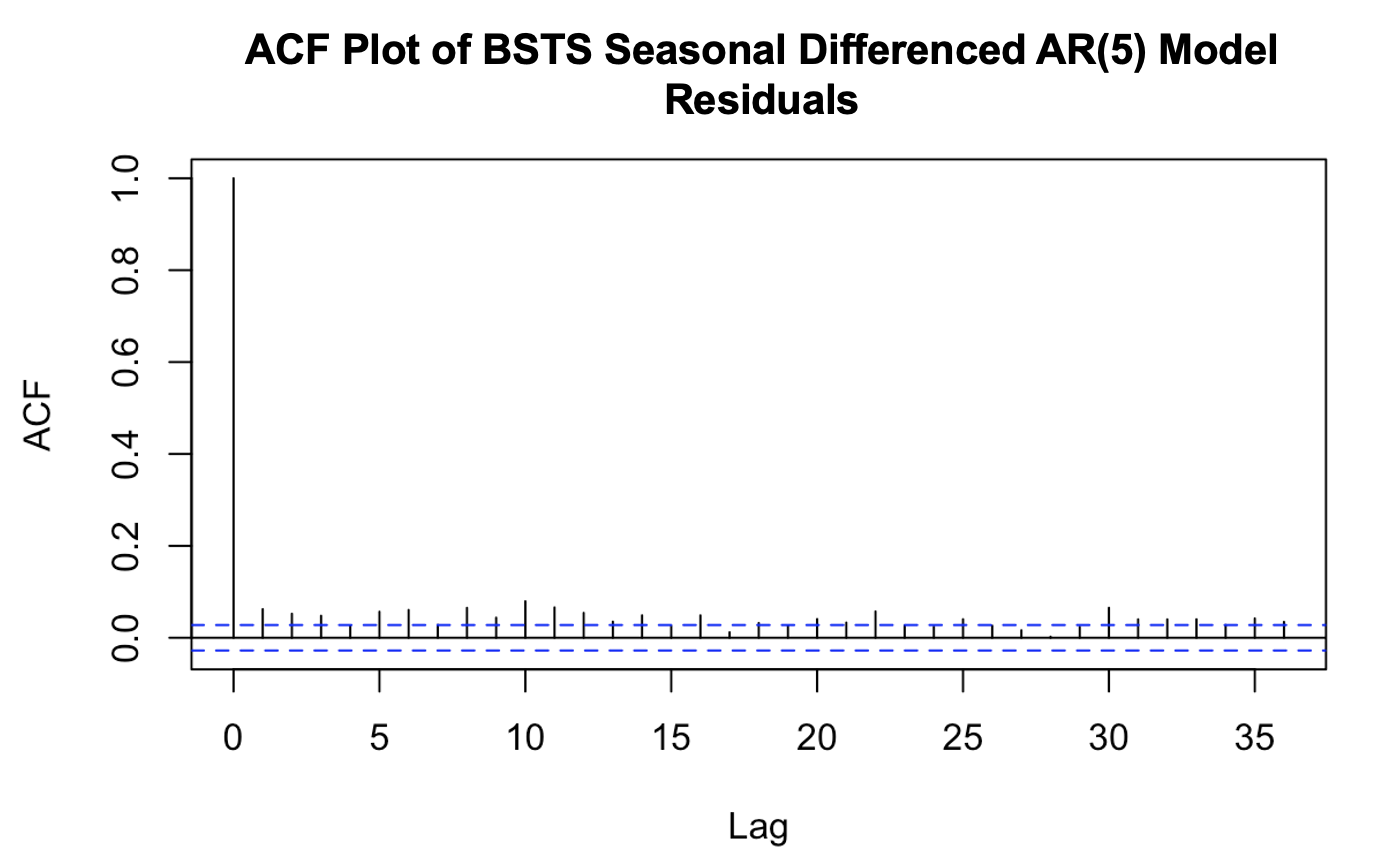
\includegraphics{BSTS_SC/bsts_season_ar.png}

\subsection{3.4 LSTM}\label{lstm}

We used LSTM because it outperforms traditional models for complex,
nonlinear time series data, especially when long-term dependencies
exist. We created a stacked model with double layer LSTM for learning
timeseries data and two dense layers for predicting output, and our
sequence window was for 60 days. The model was trained for 5 epochs and
gave great predictions.

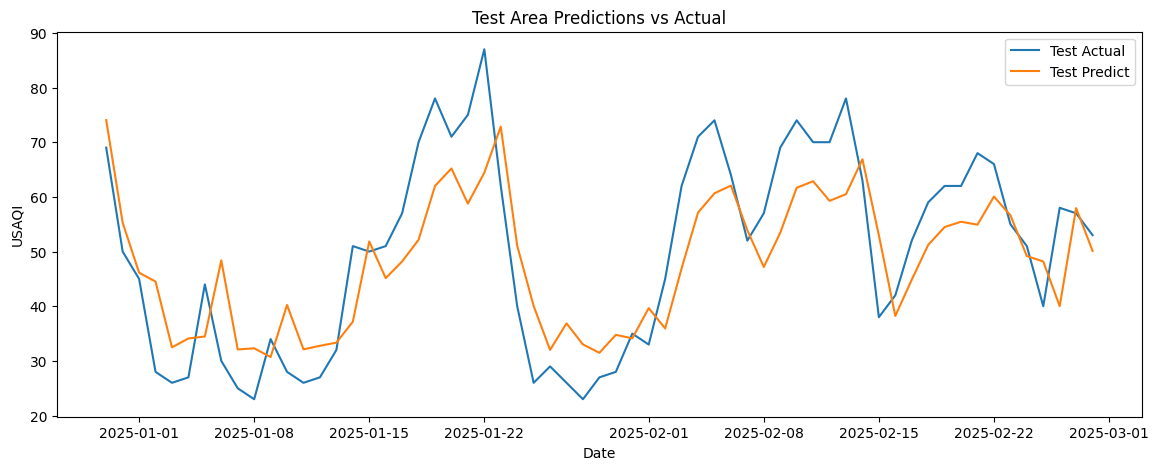
\includegraphics{lstm_plot.png}

The prediction residuals are non-correlated, which also indicates that
it is a good model.

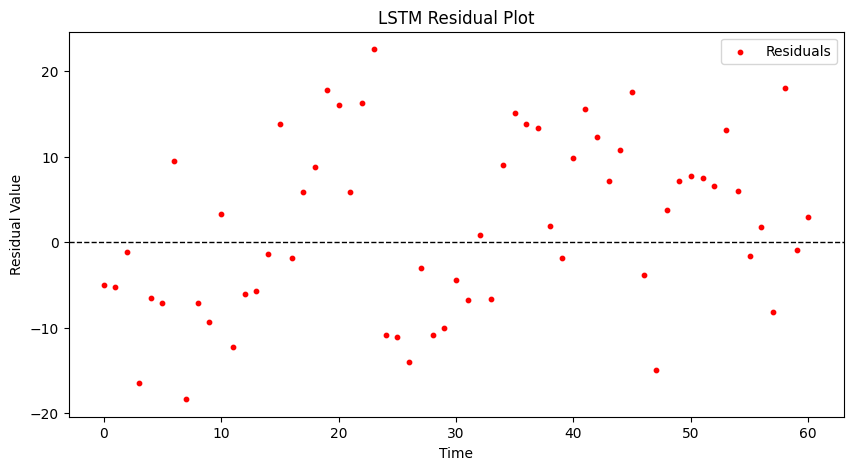
\includegraphics{lstm_resid.png}

We evaluated our model with RMSE, and had better results compared to
other simpler models. Train RMSE: 11.4 Test RMSE: 10.2 Train MAE: 8.7
Test MAE: 8.7 Train MAPE: 19.5 Test MAPE: 19.5

Our LSTM model also outperforms when evaluated against the Naïve
Persistence base model, which is simply assuming the next value to be
same as today's value. Naive Persistence Model RMSE: 10.6 Naive
Persistence Model MAE: 8.4 Naive Persistence Model MAPE: 19.2

\section{4. Results}\label{results}

\section{5. Discussion}\label{discussion}

\end{document}
